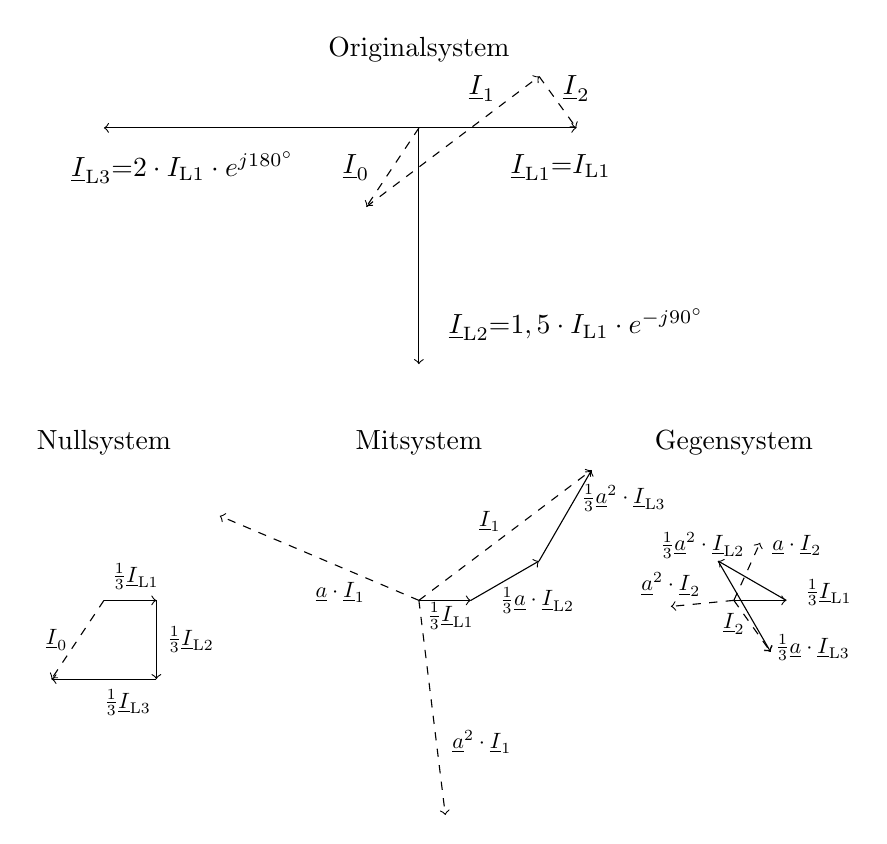
\begin{tikzpicture}
    \draw [->] (0, 0) -- (2, 0);
    \draw [->] (0, 0) -- (-4, 0);
    \draw [->] (0, 0) -- (0, -3);
    \draw [->] [dashed] (0, 0) -- (-0.666, -1);
    \draw [->] [dashed] (-0.666, -1) -- (1.527, 0.654);
    \draw [->] [dashed] (1.527, 0.654) -- (2, 0);

    \draw (1.8, -0.5) node {$\underline{I}_{\mathrm{L1}}{=}I_\mathrm{L1}$};
    \draw (-3, -0.5) node {$\underline{I}_{\mathrm{L3}}{=}2\cdot I_\mathrm{L1}\cdot e^{j180^{\circ}}$};
    \draw (2, -2.5) node {$\underline{I}_{\mathrm{L2}}{=}1,5\cdot I_\mathrm{L1}\cdot e^{-j90^{\circ}}$};
    \draw (0.8, 0.5) node {$\underline{I}_{\mathrm{1}}$};
    \draw (2, 0.5) node {$\underline{I}_{\mathrm{2}}$};
    \draw (-0.8, -0.5) node {$\underline{I}_{\mathrm{0}}$};

    \draw [->] [dashed] (0, -6) -- (2.193, -4.346);
    \draw [->] [dashed] (0, -6) -- (-2.529, -4.927);
    \draw [->] [dashed] (0, -6) -- (0.336, -8.726);
    \draw [->] (0, -6) -- (0.66, -6);
    \draw [->] (0.66, -6) -- (1.526, -5.5);
    \draw [->] (1.526, -5.5) -- (2.193, -4.346);

    \draw (0.9, -5) node [scale=0.8] {$\underline{I}_{\mathrm{1}}$};
    \draw (-1, -5.9) node [scale=0.8] {$\underline{a}\cdot\underline{I}_{\mathrm{1}}$};
    \draw (0.8, -7.8) node [scale=0.8] {$\underline{a}^2\cdot\underline{I}_{\mathrm{1}}$};
    \draw (0.4, -6.2) node [scale=0.8] {$\frac{1}{3}\underline{I}_{\mathrm{L1}}$};
    \draw (2.6, -4.7) node [scale=0.8] {$\frac{1}{3}\underline{a}^2\cdot\underline{I}_{\mathrm{L3}}$};
    \draw (1.5, -6) node [scale=0.8] {$\frac{1}{3}\underline{a}\cdot\underline{I}_{\mathrm{L2}}$};

    \draw [->] [dashed] (4, -6) -- (4.333, -5.268);
    \draw [->] [dashed] (4, -6) -- (4.467, -6.654);
    \draw [->] [dashed] (4, -6) -- (3.2, -6.077);
    \draw [->] (4, -6) -- (4.666, -6);
    \draw [->] (4.666, -6) -- (3.8, -5.5);
    \draw [->] (3.8, -5.5) -- (4.467, -6.654);

    \draw (4, -6.3) node [scale=0.8] {$\underline{I}_{\mathrm{2}}$};
    \draw (4.8, -5.3) node [scale=0.8] {$\underline{a}\cdot\underline{I}_{\mathrm{2}}$};
    \draw (3.2, -5.8) node [scale=0.8] {$\underline{a}^2\cdot\underline{I}_{\mathrm{2}}$};
    \draw (5.2, -5.9) node [scale=0.8] {$\frac{1}{3}\underline{I}_{\mathrm{L1}}$};
    \draw (3.6, -5.3) node [scale=0.8] {$\frac{1}{3}\underline{a}^2\cdot\underline{I}_{\mathrm{L2}}$};
    \draw (5, -6.6) node [scale=0.8] {$\frac{1}{3}\underline{a}\cdot\underline{I}_{\mathrm{L3}}$};

    \draw [->] [dashed] (-4, -6) -- (-4.666, -7);
    \draw [->] (-4, -6) -- (-3.334, -6);
    \draw [->] (-3.334, -6) -- (-3.334, -7);
    \draw [->] (-3.334, -7) -- (-4.666, -7);

    \draw (-4.6, -6.5) node [scale=0.8] {$\underline{I}_{\mathrm{0}}$};
    \draw (-3.6, -5.7) node [scale=0.8] {$\frac{1}{3}\underline{I}_{\mathrm{L1}}$};
    \draw (-2.9, -6.5) node [scale=0.8] {$\frac{1}{3}\underline{I}_{\mathrm{L2}}$};
    \draw (-3.7, -7.3) node [scale=0.8] {$\frac{1}{3}\underline{I}_{\mathrm{L3}}$};


    \draw (0, 1) node {Originalsystem};
    \draw (-4, -4) node {Nullsystem};
    \draw (0, -4) node {Mitsystem};
    \draw (4, -4) node {Gegensystem};

\end{tikzpicture}%